\documentclass[border=8pt]{standalone}
\usepackage{tikz}
\usepackage{amsmath, amssymb, bm}
% UiO colour palette and shared TikZ styles for thesis flowchart figures.
% Input by every standalone TikZ figure in this directory.

% UiO colours
\definecolor{uioblue1}{RGB}{62, 49, 214}
\definecolor{uioblue2}{RGB}{134, 164, 247}
\definecolor{uioblue3}{RGB}{230, 236, 255}
\definecolor{uiogreen1}{RGB}{46, 196, 131}
\definecolor{uiogreen2}{RGB}{108, 225, 171}
\definecolor{uiogreen3}{RGB}{206, 255, 223}
\definecolor{uioorange1}{RGB}{254, 161, 27}
\definecolor{uioorange2}{RGB}{253, 203, 135}
\definecolor{uioorange3}{RGB}{255, 232, 212}
\definecolor{uiopink1}{RGB}{222, 0, 0}
\definecolor{uiopink2}{RGB}{251, 102, 102}
\definecolor{uiopink3}{RGB}{254, 224, 224}
\definecolor{uioyellow}{RGB}{255, 254, 167}
\definecolor{uiogray}{RGB}{178, 179, 183}

\usetikzlibrary{arrows.meta, positioning, calc, fit, backgrounds}

% Shared styles
\tikzset{
  % Generic card with a coloured accent (#1 = base hue).
  card/.style 2 args={
    rectangle, rounded corners=3pt,
    draw=#1, line width=0.55pt,
    fill=#2,
    inner xsep=8pt, inner ysep=7pt,
    align=center,
    font=\small,
    text=black!85,
  },
  card-blue/.style  ={card={uioblue1}{uioblue3}},
  card-green/.style ={card={uiogreen1}{uiogreen3}},
  card-orange/.style={card={uioorange1}{uioorange3}},
  card-pink/.style  ={card={uiopink1}{uiopink3}},
  card-gray/.style  ={card={black!55}{black!4}},
  % Central focus body (heavier border, white fill).
  hub/.style={
    rectangle, rounded corners=8pt,
    draw=black!75, line width=0.9pt,
    fill=white,
    inner xsep=10pt, inner ysep=10pt,
    align=center,
    font=\small,
  },
  % Title text on each card.
  card-title/.style={font=\small\bfseries, text=black!85},
  % Arrows.
  flow/.style 2 args={
    -{Stealth[length=2.2mm, width=1.8mm]},
    line width=0.8pt,
    draw=#1,
    color=#1,
  },
  flow-blue/.style   ={flow={uioblue1}{uioblue1}},
  flow-green/.style  ={flow={uiogreen1!85!black}{uiogreen1!85!black}},
  flow-orange/.style ={flow={uioorange1!90!black}{uioorange1!90!black}},
  flow-pink/.style   ={flow={uiopink1}{uiopink1}},
  flow-gray/.style   ={flow={black!55}{black!55}},
  % Edge labels — small, white background, role colour.
  edge-label/.style={
    font=\scriptsize,
    fill=white, inner xsep=2pt, inner ysep=1pt,
  },
}


\begin{document}
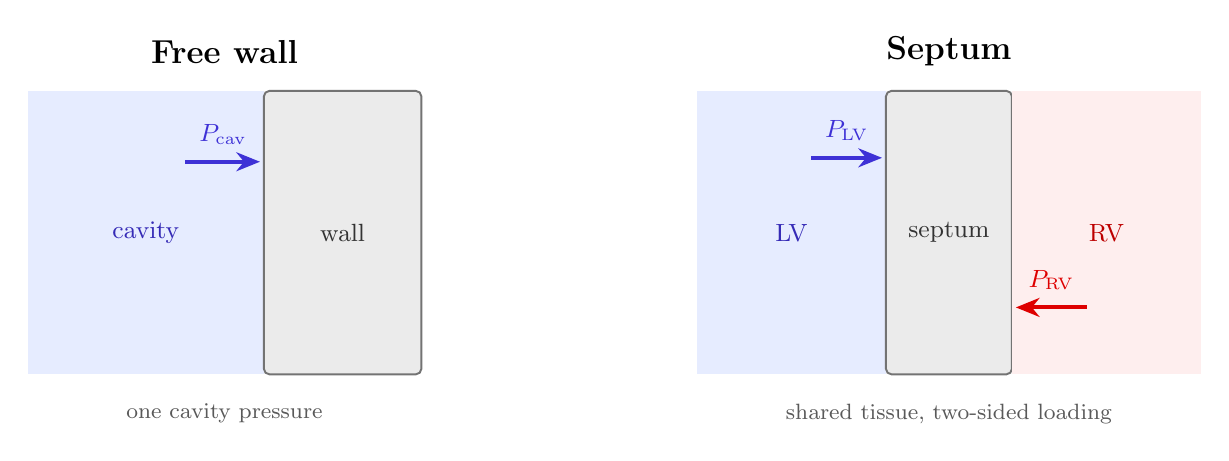
\begin{tikzpicture}[
    every node/.append style={font=\small},
  ]

  \tikzset{
    cavity-lv/.style={fill=uioblue3, draw=none},
    cavity-rv/.style={fill=uiopink3!55!white, draw=none},
    wall-box/.style={
      fill=black!8, draw=black!55, line width=0.7pt,
      rounded corners=2pt,
    },
    pressure-lv/.style={
      -{Stealth[length=3mm, width=2.4mm]},
      line width=1.4pt, color=uioblue1,
    },
    pressure-rv/.style={
      -{Stealth[length=3mm, width=2.4mm]},
      line width=1.4pt, color=uiopink1,
    },
    paneltitle/.style={font=\large\bfseries},
    panelcaption/.style={font=\footnotesize, text=black!65, align=center},
    axislabel/.style={font=\scriptsize, text=black!60},
  }

  %% ---------------- FREE WALL PANEL ----------------
  \begin{scope}
    % cavity (LV-coloured)
    \fill[cavity-lv] (0, 0) rectangle (3.0, 3.6);
    % wall
    \draw[wall-box] (3.0, 0) rectangle (5.0, 3.6);
    % in-panel labels
    \node[text=uioblue1!85!black] at (1.5, 1.8) {cavity};
    \node[text=black!80] at (4.0, 1.8) {wall};
    % pressure arrow into wall
    \draw[pressure-lv] (2.0, 2.7) -- (2.95, 2.7);
    \node[text=uioblue1, above=0pt] at (2.48, 2.8) {$P_\text{cav}$};
    % panel title and caption
    \node[paneltitle] at (2.5, 4.1) {Free wall};
    \node[panelcaption] at (2.5, -0.5) {one cavity pressure};
  \end{scope}

  %% ---------------- SEPTUM PANEL ----------------
  \begin{scope}[xshift=8.5cm]
    % LV cavity
    \fill[cavity-lv] (0, 0) rectangle (2.4, 3.6);
    % septum
    \draw[wall-box] (2.4, 0) rectangle (4.0, 3.6);
    % RV cavity
    \fill[cavity-rv] (4.0, 0) rectangle (6.4, 3.6);
    % in-panel labels
    \node[text=uioblue1!85!black] at (1.2, 1.8) {LV};
    \node[text=black!80] at (3.2, 1.8) {septum};
    \node[text=uiopink1!85!black] at (5.2, 1.8) {RV};
    % LV pressure arrow into septum (upper)
    \draw[pressure-lv] (1.45, 2.75) -- (2.35, 2.75);
    \node[text=uioblue1, above=0pt] at (1.9, 2.85) {$P_\text{LV}$};
    % RV pressure arrow into septum (lower)
    \draw[pressure-rv] (4.95, 0.85) -- (4.05, 0.85);
    \node[text=uiopink1, above=0pt] at (4.5, 0.95) {$P_\text{RV}$};
    % panel title
    \node[paneltitle] at (3.2, 4.1) {Septum};
    \node[panelcaption] at (3.2, -0.5) {shared tissue, two-sided loading};
  \end{scope}

\end{tikzpicture}
\end{document}
